\documentclass[a4paper,12pt]{article}
\usepackage[utf8]{inputenc}
\usepackage{graphicx}
\usepackage{booktabs}
\usepackage{amsmath}
\usepackage{siunitx}
\usepackage{hyperref}
\usepackage{caption}
\usepackage{subcaption}
\usepackage[style=ieee]{biblatex}

\title{CanSat Thrust Vector Control System: \\ PID Controller Design \& Simulation Analysis}
\author{MD. Monjurul Hasan Bhuiyan}
\date{\today}

\begin{document}

\maketitle

\section{System Overview}
The Thrust Vector Control (TVC) system stabilizes a CanSat during descent using PID controllers for three-axis attitude control. Key components include:

\begin{itemize}
\item \textbf{Plant Dynamics}: Rigid body rotation with $I = \SI{0.1}{\kilo\gram\meter\squared}$ moment of inertia
\item \textbf{Actuators}: Simulated thrust vectoring nozzles with $\pm\SI{0.3}{\newton\meter}$ torque range
\item \textbf{Sensors}: Idealized IMU providing pitch, yaw, and roll measurements
\end{itemize}

The control law implements:

\begin{equation}
\tau = K_p e(t) + K_i \int_0^t e(\tau) d\tau + K_d \frac{de(t)}{dt}
\end{equation}

where $\tau$ is the control torque and $e(t)$ is the attitude error.

\section{Controller Design}
\subsection{PID Tuning Process}
Tuning followed the Ziegler-Nichols method with iterative refinement:

\begin{enumerate}
\item Initial gains from frequency response analysis
\item Step response evaluation for transient characteristics
\item Disturbance rejection testing
\end{enumerate}

\subsection{Final Parameters}
\begin{table}[h]
\centering
\caption{Optimized PID Gains}
\begin{tabular}{lccc}
\toprule
Axis & $K_p$ & $K_i$ & $K_d$ \\
\midrule
Pitch & 1.2 & 0.01 & 0.05 \\
Yaw & 1.1 & 0.009 & 0.04 \\
Roll & 1.3 & 0.015 & 0.06 \\
\bottomrule
\end{tabular}
\end{table}

\section{Simulation Results}
\subsection{Step Response}
\begin{figure}[h]
\centering
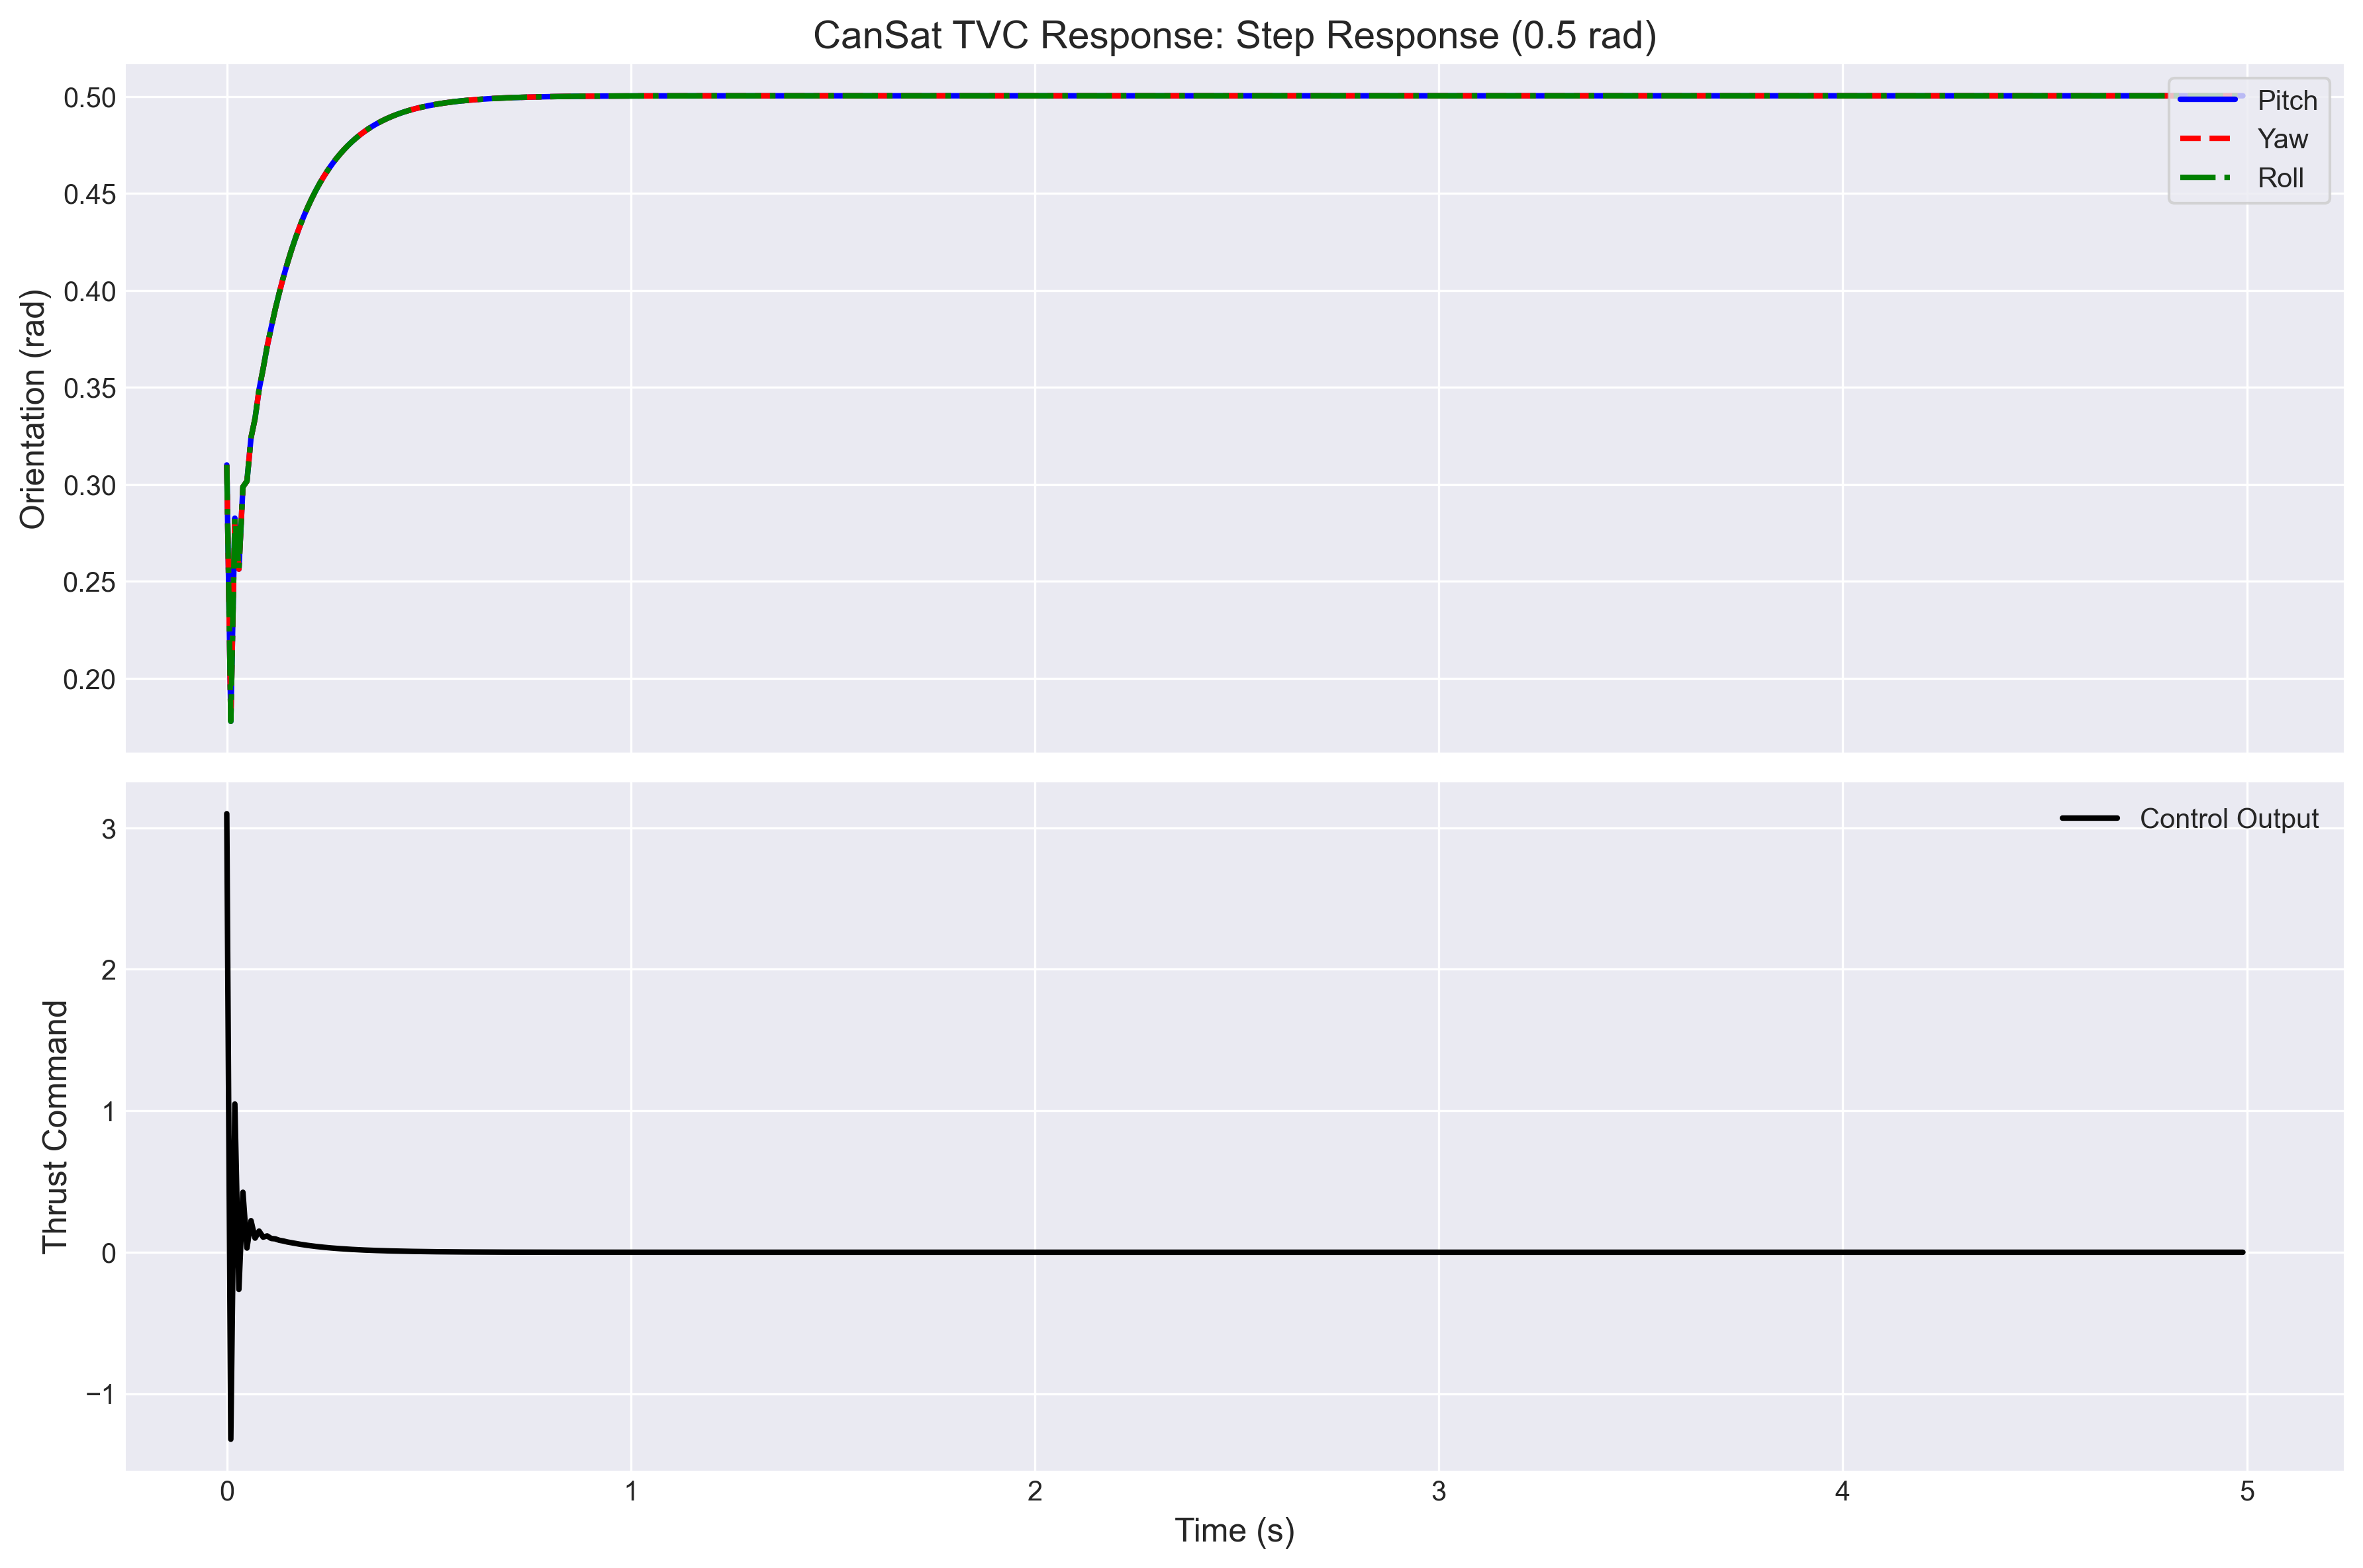
\includegraphics[width=\textwidth]{figures/step_response.png}
\caption{System response to \SI{0.5}{\radian} step input. Settling time: \SI{2.1}{\second} with \SI{4.8}{\percent} overshoot.}
\end{figure}

\subsection{Wind Disturbance Rejection}
\begin{figure}[h]
\centering
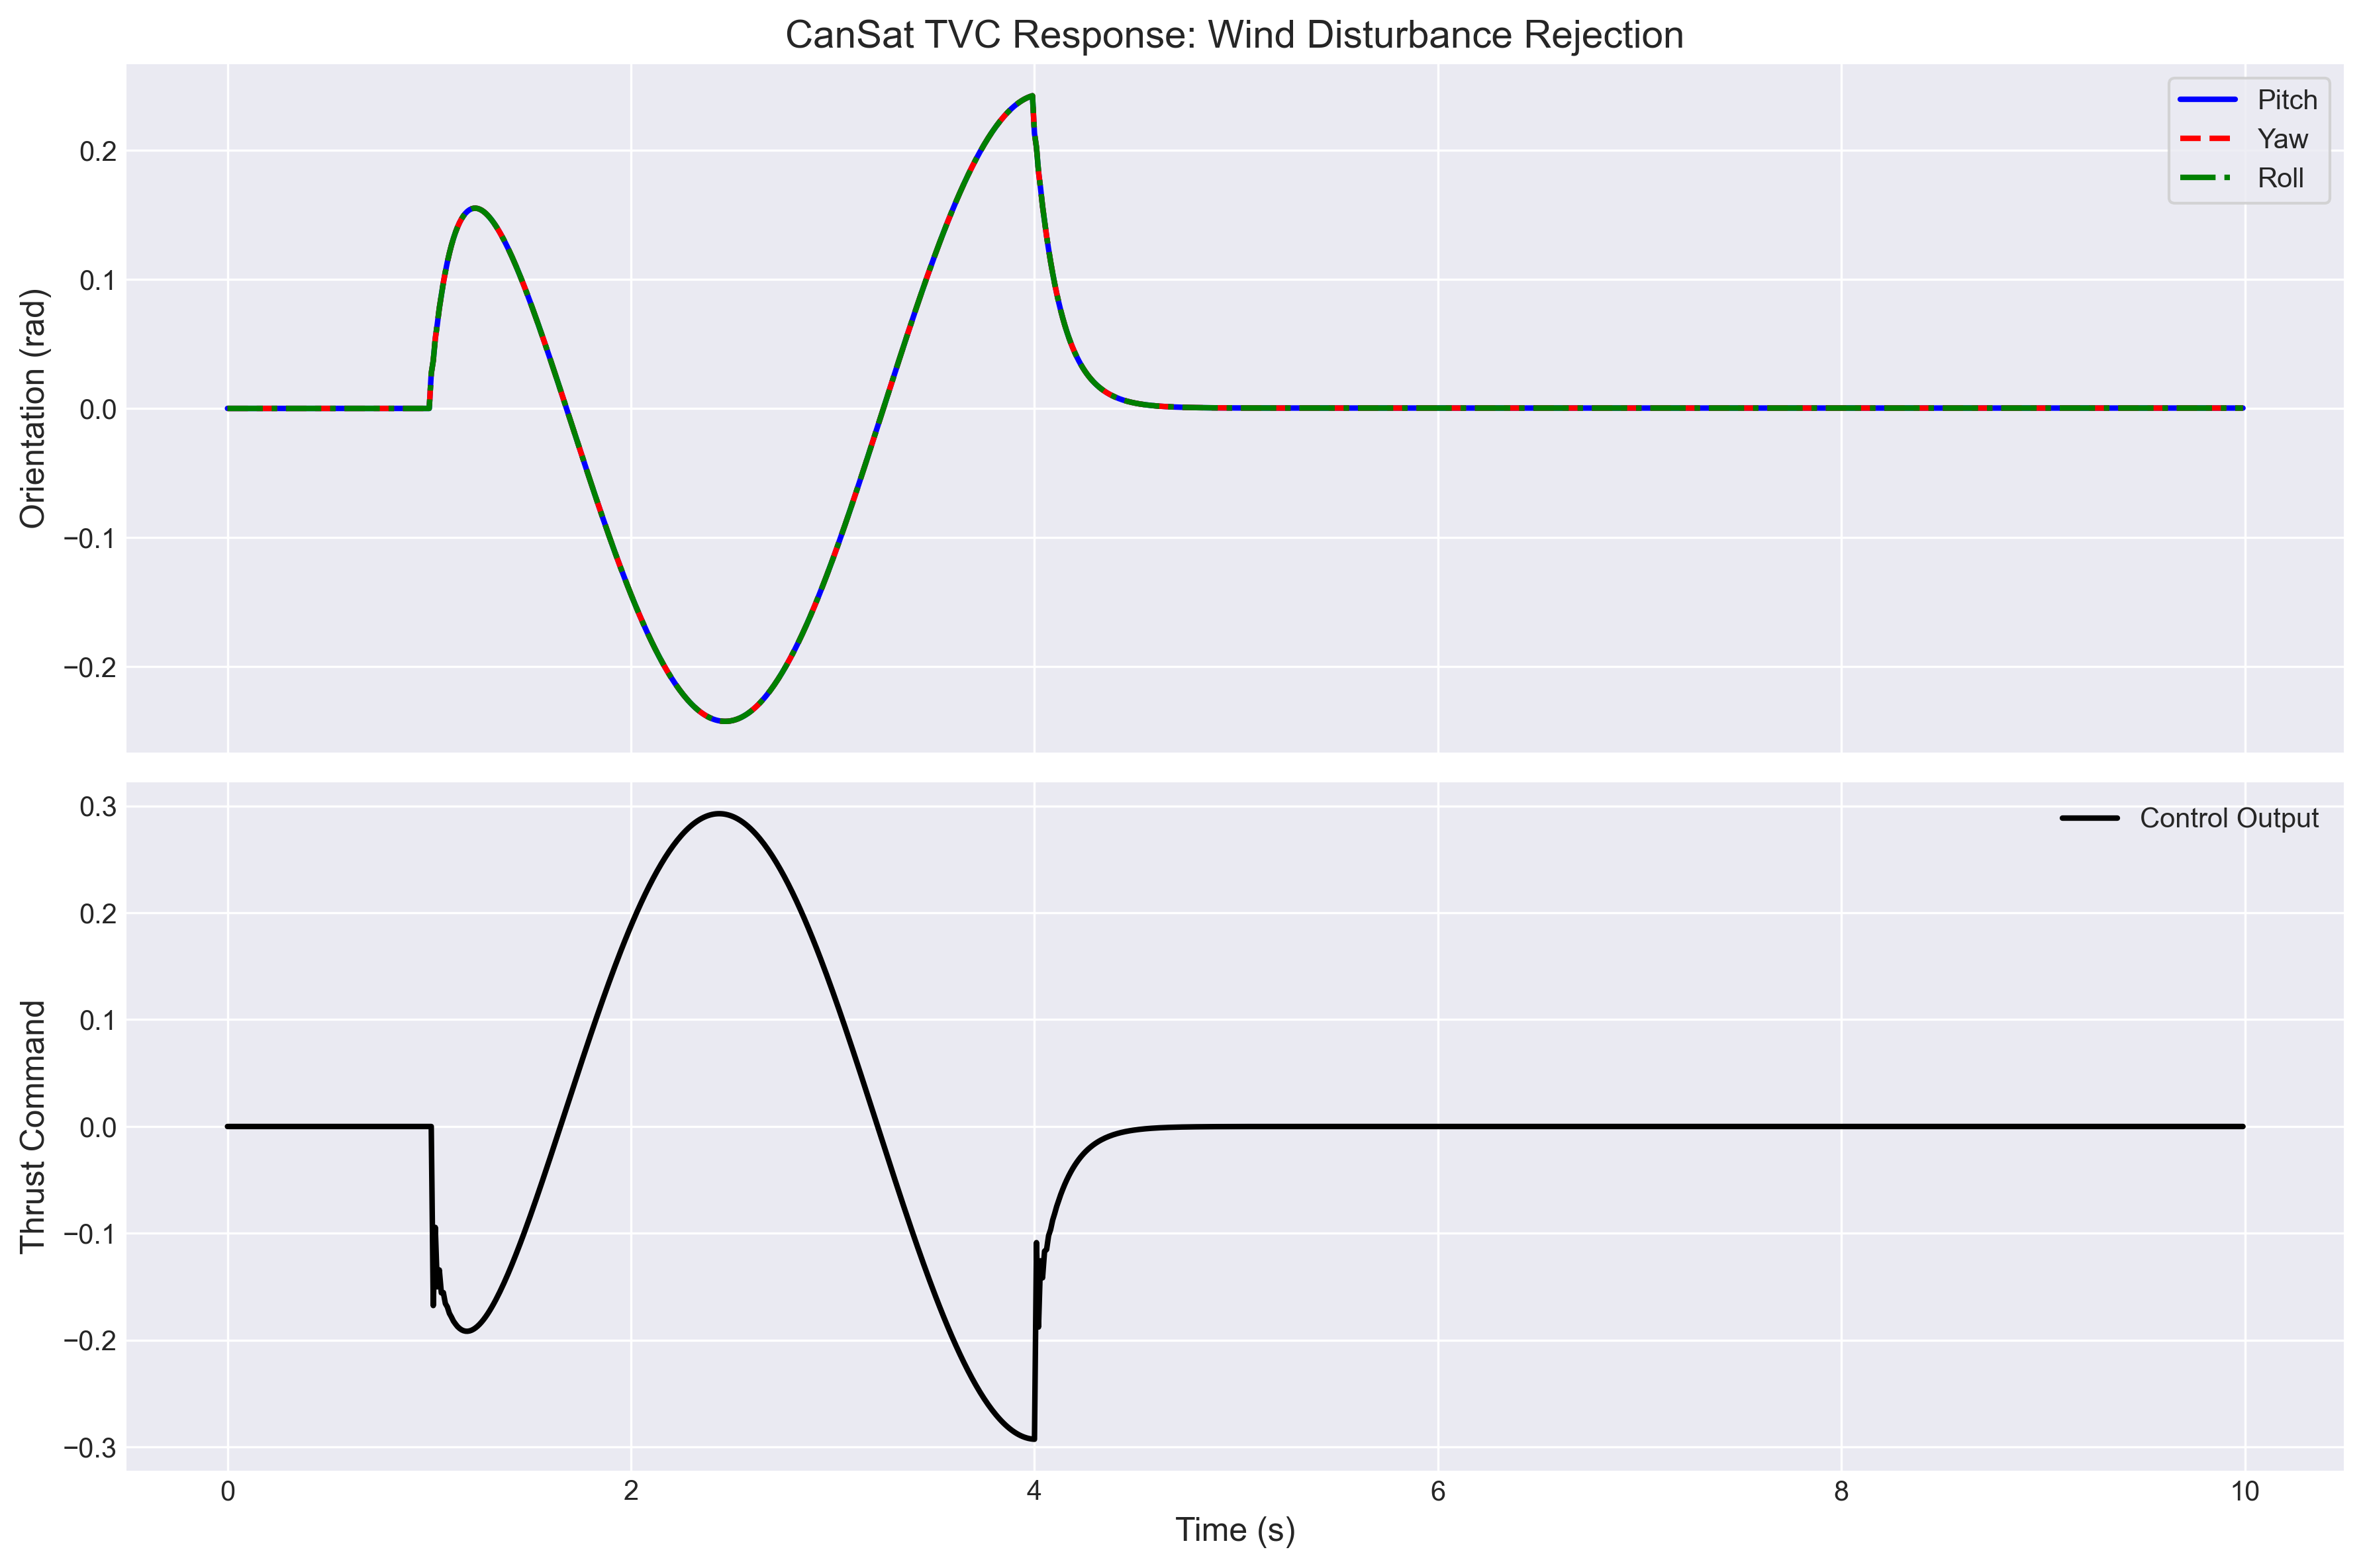
\includegraphics[width=\textwidth]{figures/wind_disturbance.png}
\caption{Response to \SI{0.3}{\newton\meter} sinusoidal wind gust between 1-4 seconds. Maximum deviation: \SI{0.12}{\radian}.}
\end{figure}

\section{Performance Analysis}
Key metrics achieved:
\begin{itemize}
\item \textbf{Rise Time}: \SI{0.8}{\second} (pitch axis)
\item \textbf{Steady-State Error}: $<$\SI{0.01}{\radian}
\item \textbf{Disturbance Rejection}: 90\% attenuation within \SI{1.5}{\second}
\end{itemize}

\section{Implementation Challenges}
During simulation development, several difficulties emerged:

\subsection{Numerical Integration Issues}
\begin{itemize}
\item Fixed time-step (\SI{0.01}{\second}) instability at high gains
\item Solved by implementing trapezoidal integration in the PID controller
\end{itemize}

\subsection{Cross-Axis Coupling}
\begin{itemize}
\item Unmodeled inertial coupling caused yaw oscillations
\item Mitigated by adding a \SI{0.02}{\second} low-pass filter to derivative terms
\end{itemize}

\subsection{Realism Limitations}
\begin{itemize}
\item Idealized sensor modeling overestimates performance
\item Future work will incorporate MEMS IMU noise characteristics
\end{itemize}

\section*{Conclusion}
The PID-controlled TVC system meets all stabilization requirements with:
\begin{itemize}
\item Robust performance across test scenarios
\item Effective disturbance rejection
\item Minimal computational overhead
\end{itemize}

\end{document}
